\chapter{The Steve Tutorial} \label{ch:tutorial}

% It might be worthwhile to divide this into three major sections:
%
% 1. General purpose computing
% 2. Packet specification
% 3. Pipeline specification
%    - decoders
%    - flow tables

The primary focus of the Steve Programming Language is to provide features for
defining and connecting the pipeline processing stages described in Chapter
\ref{ch:pipeline_model}. This chapter will explain how a user writes each of these
components. Specifically, this chapter will discuss how headers are represented, how to
write decoders, how to write tables, and how to apply actions to packets.

By the end of this chapter, a user should be able to write many basic network
applications using Steve. Four such applications will be presented in Section \ref{tut:examples}: a simple MAC
learning switch, an IPv4 learning switch, a stateless TCP/UDP firewall, and a wire. Many of the examples
presented throughout this chapter are just smaller parts of these applications
presented in isolation. This tutorial will slowly build
up these little components and explain what they do before finally presenting
the complete program at the end.

Semantics and limitations of Steve will be mentioned throughout this chapter, 
but only in minor detail. For the complete semantic description of
Steve, including grammar, typing rules, and other restrictions, see the Reference Guide in Chapter \ref{ch:users_guide}. For a complete reference of all Steve
grammar, see Appendix \ref{ap:a}.

\section{General Purpose Language Features} \label{tut:gen_purp}

Steve supports language features that can be considered
\textit{general purpose}. These language features are common to most programming
languages and are not explicitly for packet processing, though they may prove
useful.

\subsection{Variables} \label{tut:variable}

Steve allows for the allocation of both local and global variables for storing values. Suppose one wanted to write a variable named \texttt{x} which holds an
integer value \texttt{10}. It would be written as follows.

\begin{codepage}
\begin{lstlisting}
var x : int = 10;
\end{lstlisting}
\end{codepage}

The type of the variable, \texttt{int}, follows the colon
(\texttt{:}). A new value can be assigned to it.

\begin{codepage}
\begin{lstlisting}
x = 1;
\end{lstlisting}
\end{codepage}

Arithmetic and bitwise operations can be performed as well. The complete set of
arithmetic and bitwise operations can be found in Section
\ref{guide:binary_expr}.

\begin{codepage}
\begin{lstlisting}
var y : int = 2;
var z : int = 3;
y = x + y; // Addition
z = y + z + 1;
z = z << 4; // Left shift
var a : int = y & z; // Bitwise and
\end{lstlisting}
\end{codepage}


\subsection{Conditional Statements} \label{tut:condition}

Steve supports three conditional statements for decision making: the \texttt{if} statement and the \texttt{match} statement. The \texttt{if} statement is the same as most C-like languages.

\begin{codepage}
\begin{lstlisting}
var a : bool = true;
var b : bool = false;

// If statement
if (a || b) { }

// If else statement
if (a && b) { ... }
else if (a) { ... }
else { ... }
\end{lstlisting}
\end{codepage}

A \texttt{match} statement allows for a decision to be made given a number of possible
case values. This makes it similar to a C-like switch statement, with the only
major difference being that there is no \textit{fall-through} behavior. In other
words, after the execution of a \texttt{case} statement, control jumps out of the \texttt{match}
statement rather than moving to the next case (i.e. an implied \texttt{break}). The
condition and labels must be integers just like in C. A \texttt{match} statement can be
written as follows.

\begin{codepage}
\begin{lstlisting}
// Assuming there are integer variables named x and y.
match (x) {
  case 0: x = x + 1;
  // Multiple statements following the label must be
  // enclosed in a block.
  case 1: {
    x = x + 2;
    y = y * x;
  }

  // The default case statement.
  miss: x = 0;
}
\end{lstlisting}
\end{codepage}

Here, if \texttt{x} equals \texttt{0}, then \texttt{x = x + 1} gets executed. If
\texttt{x} equals \texttt{1}, then two statements get executed in order:
\texttt{x = x + 2}, then \texttt{y = y * x}. If \texttt{x} is neither, then
\texttt{x = 0} is executed.

\subsection{While Loops} \label{tut:while}

The \texttt{while} loop appears in Steve just like they appear in C-like languages. 
They also support the \texttt{break} and \texttt{continue} statements for limited
branching abilities inside a loop.

The following is a trivial \texttt{while} loop which demonstrates the basics
of \texttt{break} and \texttt{continue}. By the end of this loop, the value of \texttt{x} will be \texttt{4} and \texttt{z} will be \texttt{2}.

\begin{codepage}
\begin{lstlisting}
var x : int = 0;
var z : int = 0;
// Loop while x is less than 5.
while (x < 5) {
  x = x + 1;
  // If x equals 3, control goes back to the
  // first statement in the loop body.
  if (x == 3)
    continue;

  // This part is never reached if x == 2.
  // If z equals 2, then we exit the loop
  // altogether.
  if (z == 2)
    break;
  // This will never execute when z == 2.
  z = z + 1;
}
\end{lstlisting}
\end{codepage}

The usage of \texttt{while} loops in packet processing right now is rather limited. Usage
of loops will rarely come up in defining pipeline processing stages. However,
they may become more useful as other features are added.

\subsection{Functions} \label{tut:function}

Steve supports writing simple functions, though the syntax is a little different
from C-like languages. Functions can be called with parameters and can return
results just like any other language.

Suppose one wanted to write a function named \texttt{sum} which takes two
integers, \texttt{a} and \texttt{b}, and returned the integer sum of \texttt{a}
and \texttt{b}. One would write \texttt{sum} as follows.

\begin{codepage}
\begin{lstlisting}
def sum(a : int, b : int) -> int
{
  return a + b;
}
\end{lstlisting}
\end{codepage}

The return type follows the \texttt{->} in Steve functions. To call
the \texttt{sum} function one would write the following. Here, the result of
\texttt{sum} would be \texttt{3}.

\begin{codepage}
\begin{lstlisting}
var x : int = 1;
var y : int = 2;
var z : int = sum(x, y);
\end{lstlisting}
\end{codepage}

\subsection{Literals} \label{tut:literal}

% FIXME: I would give a list of the literal kinds first and then talk
% about digit separators. So... Here is a hex literal. Here is a binary
% literal. Look, you can use digit separators!

Steve supports decimal, binary, and hexadecimal integer literals. Steve does not
currently support things like IP address literals or MAC address literals.

Hexadecimal literals all start with the prefix \texttt{0x} followed by any
number of digits between \texttt{0} and \texttt{9}. Binary literals all start with the prefix \texttt{0b} followed by any number of
\texttt{0}'s and \texttt{1}'s.

These integer literals can be written as follows.

\begin{codepage}
\begin{lstlisting}
17 // Decimal literal
0x11 // Hexadecimal 17
0x00010001 // Binary 17
\end{lstlisting}
\end{codepage}
 
The underscore (\texttt{\_}) can optionally be used as a digit separator for hexadcimal and binary literals with no impact on the value of that literal.
This is purely for organization and readability.

\begin{codepage}
\begin{lstlisting}
// These are the same binary value.
0b10101010
0b1010_1010

// These are the same hexadecimal value.
0x0800
0x08_00
\end{lstlisting}
\end{codepage}

\section{Layouts} \label{tut:layout}

A \textit{layout} is used to describe the \textit{structure} of a packet header.
More specifically, they describe \textit{what} fields are present, their
\textit{lengths}, the \textit{order} in which they appear, and their
\textit{relative offset} from the beginning of the header. Layouts become
pivotal during decoding stages, where all this information is used to guide the
extraction of fields from a header.

\textit{A layout and a header are two different concepts.}
It is important to make this distinction clear. A layout is like a blueprint for
a header. It gives us information; it \textit{describes} that header. The header
is an actual sequence of bits, a portion of the packet, which is taken off of the
network. The header \textit{exists} whereas a layout helps the Steve application
\textit{understand} it.

The simplest example to begin with is the
ethernet header \cite{eth_std}. Ethernet is a Layer 2 protocol
and the most common in use. The first header most programs decode will be
ethernet.

An ethernet header has three fields: destination and source MAC addresses which
are both 6 bytes (or 48-bits) long, and a type field which is 2 bytes (or
16-bits long). A layout describing the ethernet header is written using a
\textit{layout declaration} (\ref{guide:layout}). The following example presents
an ethernet layout declaration matching these specifications.

\begin{codepage}
\begin{lstlisting}
// This layout describes the ethernet header.
layout ethernet {
	dst  : uint(48); // This is 48 bits long.
	src  : uint(48); // This is 48 bits long.
	type : uint(16); // This is 16 bits long.
}
\end{lstlisting}
\end{codepage}

Here, a layout named \texttt{ethernet} is declared. Each layout defines which
fields it has with a \textit{field declarations} (\ref{guide:layout}). Each
field is given a \textit{name} (\ref{guide:identifiers}) and a \textit{type}
(\ref{guide:type}). In this example, three such fields are declared: \texttt{dst},
\texttt{src}, and \texttt{type}. The \textit{length} of each field is denoted by
the \textit{size} required to store an object of that \textit{type}. Here, each
field has unsigned integer type (\ref{guide:integer_type}), \texttt{uint}, with
an (optional) precision. The precision denotes the size (in bits) needed to
store that integer. Thus the \texttt{dst} and \texttt{src} fields have a length
of 48 bits, and the \texttt{type} field has a length of 16 bits.

The \textit{relative offset} of each field is the number of bytes it is away
from the beginning of the header. The first field will always have a relative
offset of 0 bytes. The relative offset of each subsequent field is equal to the
sum of the lengths of all fields preceding it. Here, \texttt{dst} has a relative
offset of 0 bytes, \texttt{src} has one of 6 bytes, and \texttt{type} has one of
12 bytes.

Here, the fields appear in the order with which they would normally appear
in an ethernet header. This is important. Field ordering should always be
preserved when declaring layouts. If the ordering is incorrect, decoders will
assume a sequence of bits is a certain field when it truly is not.

Not all header structures are as simple as the ethernet header. Sometimes one
must deal with headers nested inside headers. It is for this very reason, that
Steve allows layouts to be nested.

The following presents such a case where the programmer expects a VLAN header
\cite{vlan_std} nested before the \texttt{type} field of an ethernet
header.

\begin{codepage}
\begin{lstlisting}
// Layouts may be nested like this.
layout ethernet {
  dst  : uint(48);
  src  : uint(48);
  vlan_tag : vlan; // Nested layout
  type : uint(16);
}

layout vlan {
  type : uint(16);
  tci  : uint(16);
}
\end{lstlisting}
\end{codepage}

In this example, two layouts are declared: \texttt{ethernet} and \texttt{vlan}. To
achieve a nested layout a field named \texttt{vlan\_tag} is added to
\texttt{ethernet} and its type is given as the name of another layout,
\texttt{vlan}. The length of the \texttt{vlan\_tag} field would be the sum of
its sub-fields, in this case, 32 bits or 4 bytes.

With the way
layouts are described and written, it is easy to draw the comparison between layouts and
classes in object-oriented languages. \textit{Layouts are not the same concept as classes.} Layouts are much stricter.

First of all, \textit{the types of each field are restricted}. Fields may only
have two types: integer (\ref{guide:integer_type}) and layout
(\ref{guide:layout_type}). There may be varying kinds of integer (e.g.
precisions, signed, unsigned, etc.), but the precision of each integer must also
be \textit{byte-aligned}, that is, a multiple of 8.

Second, the most important distinction is that \textit{objects of layout type
can never be created}. Layouts may not appear as the type of parameters, nor may
they appear as return types. All of the following are considered illegal.

\begin{codepage}
\begin{lstlisting}
layout L1 { f1 : uint; f2 : uint(16); }
var x : L1 = 0; // Invalid.
// Invalid parameter type and return type.
def foo(y : L1) -> L1 { }
\end{lstlisting}
\end{codepage}

Packets and their headers exist independent of a running Steve application.
Layouts are purely used to guide decoding them. Additionally, there are a number
of concerns related to constructing objects of layout type, thus such behavior
is not allowed. For further details on layout limitations, refer to Section
\ref{guide:layout} in the Reference Guide.

Another important thing to note is that Steve does not currently support dynamically
sized types (DST). A DST is a type whose size is predicated upon some value
known only during runtime. These DST's are used to represent fields whose
lengths are dynamic. Some examples of dynamic length fields are the
\texttt{options} fields in IPv4, IPv6, and TCP headers \cite{ipv4_std, ipv6_std,
tcp_std}.

DST's are a language feature that will eventually be added, but are outside the
current implementation. Because of this, fields whose lengths are dynamic cannot
currently be declared, extracted, nor used. The existence and eventual support
of DST's is one of the reasons why objects of layout type cannot be created.
This is further discussed in Section \ref{guide:no_dst}.

The following example presents a case where some of these limitations become relevant -- the IPv4 layout. IPv4 is a Layer 3 protocol and is used
for routing. An IPv4 header appears in almost all Internet-bound packets and
thus makes it a common layout to write.

\begin{codepage}
\begin{lstlisting}
layout ipv4 {
  version_ihl : uint(8); // Non-byte aligned fields are merged.
  dscp_ecn    : uint(8);  // This is merged, too.
  len         : uint(16);
  id          : uint(16);
  fragment    : uint(16); // Fragment usually has flags.
  ttl         : uint(8);
  protocol    : uint(8);
  checksum    : uint(16);
  src         : uint(32);
  dst         : uint(32);
  // Note the missing, unsupported options field.
}
\end{lstlisting}
\end{codepage}

In this example, one can seen that \texttt{version} (a 4 bit field) has to be
merged with \texttt{ihl} (internet header length) (also a 4 bit field) to
achieve byte alignment. The same is true for \texttt{dscp} and \texttt{ecn}. The
\texttt{fragment} field, typically composed of three 1 bit flags and a 13 bit
fragment offset field, is merged into a single 16 bit field. To recover the
values of these sub-fields, one must use bitwise-and
(\ref{guide:bitwise_expr}) to mask the un-needed bits. An example will come up
later when an IPv4 decoder is discussed.

\section{Decoders} \label{tut:decoder}

Decoding stages, or \textit{decoders} for short, are special purpose functions
used to handle decoding and extracting fields from a \textit{single} header. Decoders use layouts to help them extract fields. By
chaining multiple decoders together, a user can construct a sequence of
functions used to parse an entire packet. 

When writing a decoder, it is good practice to keep the following in mind.

\begin{itemize}
\item Which header is being decoded?

\item What fields from the header are needed and why?

\item How will these fields be used? Will they be used in arithmetic or 

\item \textit{Actions} (described later in Section \ref{tut:action}) are used to manipulate packet fields, forward packets,
and add/remove flow entries from tables. What actions must be be taken on the packet?

\item Where must the packet be sent next? Must it be further decoded or can it be sent to table matching for decision making?
\end{itemize}

\subsection{The Basic Decoder Form} \label{tut:basic_decoder}

A decoder is written using a \textit{decoder declaration} (\ref{guide:decoder}).
A decoder declaration has four important parts: 1) a name, 2) a \textit{layout
rule}, 3) a keyword specifying whether this is the starting decoder, and 4) a
body.

A \textit{layout rule} is the layout which the decoder
will use to guide its extractions. It provides all the information necessary for
the decoder to determine which bits in a packet comprise which fields.

For almost all applications, ethernet will need to be decoded first. An assumption is made that all packets coming to the device begin with the
ethernet header (the most common first header). The basic ethernet decoder would look like the following example.

\begin{codepage}
\begin{lstlisting}
// The empty ethernet decoder.
decoder start eth_d(ethernet) { ... }
\end{lstlisting}
\end{codepage}

In this example, the decoder is named \texttt{eth\_d}. The layout rule is
\texttt{ethernet}. The \texttt{start} keyword has been added to denote that this is the \textit{starting decoder}. This means this
decoder will always be the first to execute. A program must have exactly one
starting decoder. 

The decoder has a body, delimited by $\lbrace\rbrace$, which executes. This body will be filled with operations for the decoder to perform.

\subsection{Extractions} \label{tut:decoder_extract}

The primary goal of a decoder is to extract fields from a single header. These
extracted fields, or \textit{extractions} for short, are found using information
gathered from the \textit{layout rule}.

To extract a field, one writes an \textit{extract declaration}
(\ref{guide:extract}) in the decoder's body. The programmer (hypothetically) makes the decision that they want all fields
extracted from the ethernet header. The decoder would thus look like the following.

\begin{codepage}
\begin{lstlisting}
// The ethernet decoder extracts all fields.
decoder start eth_d(ethernet)
{
	extract ethernet.dst;
	extract ethernet.src;
	extract ethernet.type;
}
\end{lstlisting}
\end{codepage}

Each extract declaration gives a \textit{field name} (\ref{guide:field_name}).
The field name refers to a field in the \textit{layout rule}. Here,
\texttt{ethernet.dst}, \texttt{ethernet.src}, and \texttt{ethernet.type} are
field names which refer to a respective extraction. The decoder
gathers information on these fields from the layout rule to find the relative offset and length of the field, then saves the information
in the context data structure (\ref{context_desc}) as offset-length pairs.

Only field names which refer to fields in the layout rule may be used. For example, it would not be possible to extract \texttt{ipv4.protocol} in the \texttt{eth\_d} decoder. It would
obviously make no sense to extract a field not in the header. 

\subsection{How Decoder's Extract Fields} \label{tut:extract_how}

A decoder follows a set of steps to determine the location and length of a field. A decoder has a very limited look into a packet. It only has
access to a subset of contiguous bytes, known as the \textit{view} of the
decoder. A decoder's view begins where the header it decodes begins, and ends
(implicitly) where that header ends. Its view ends implicitly because a layout
only provides information on a single header. It is obvious that a
decoder would not be able to decode past the final field it knows about from its
layout rule.

Figure \ref{fg:decoding} demonstrates how decoders and their views work. Here, the Steve application was decoding a typical packet with ethernet, IPv4, and UDP headers. The
starting decoder's view always starts at the beginning of the packet. In the
case of Figure \ref{fg:view1}, the first header is ethernet.

\begin{figure}[ht]
\begin{subfigure}[t]{.45\textwidth}
  \centering
  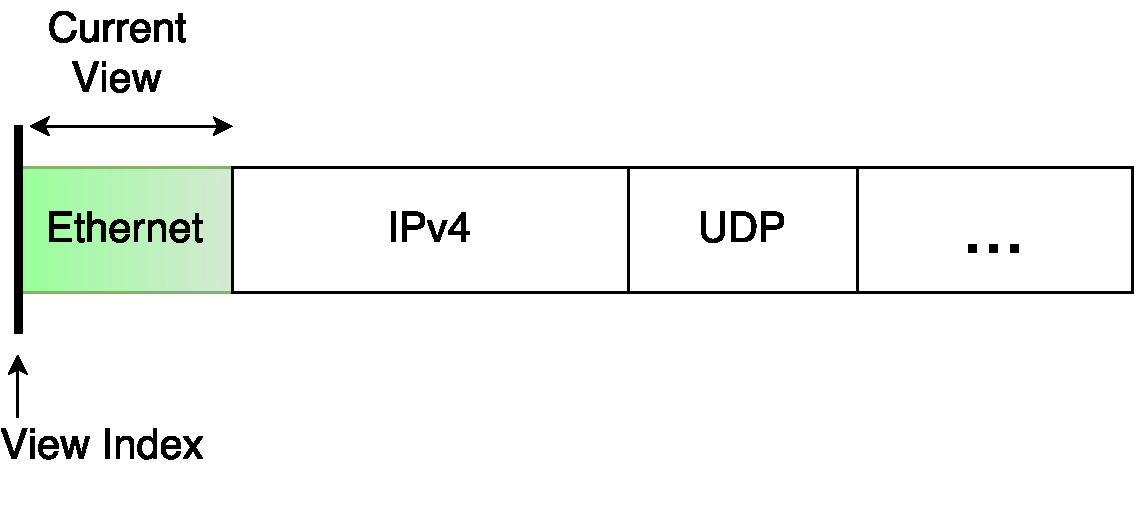
\includegraphics[width=.8\linewidth]{view1}
  \caption{The view of the starting decoder, in this case, the ethernet
decoder. The beginning of the view is the beginning of the ethernet
header, which is also the beginning of the packet.}
  \label{fg:view1}
\end{subfigure}%
\hfill
\begin{subfigure}[t]{.45\textwidth}
  \centering
  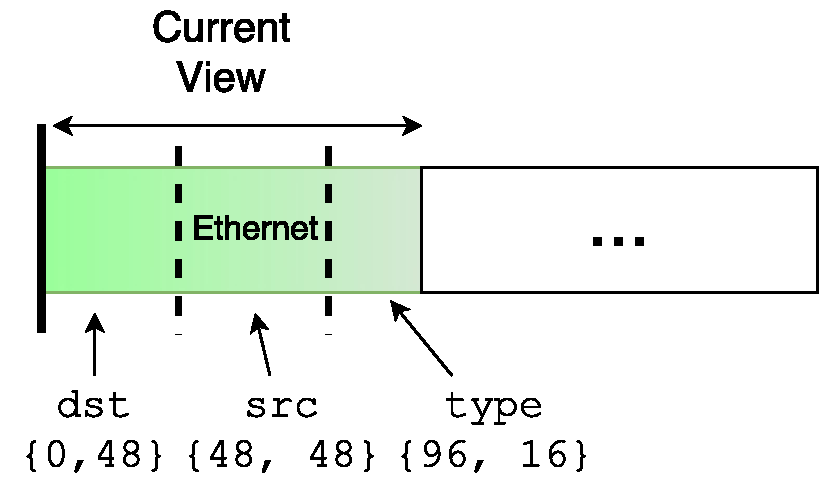
\includegraphics[width=.8\linewidth]{view2}
  \caption{The beginning of a field is discovered by its relative offset from
the beginning of the view. The end is determined by the field's length. The
field \texttt{dst} is 0 bytes from the beginning, \texttt{src} is 6 bytes in,
and \texttt{type} is 12 bytes in.}
  \label{fg:view2}
\end{subfigure}

\begin{subfigure}[t]{.45\textwidth}
  \centering
  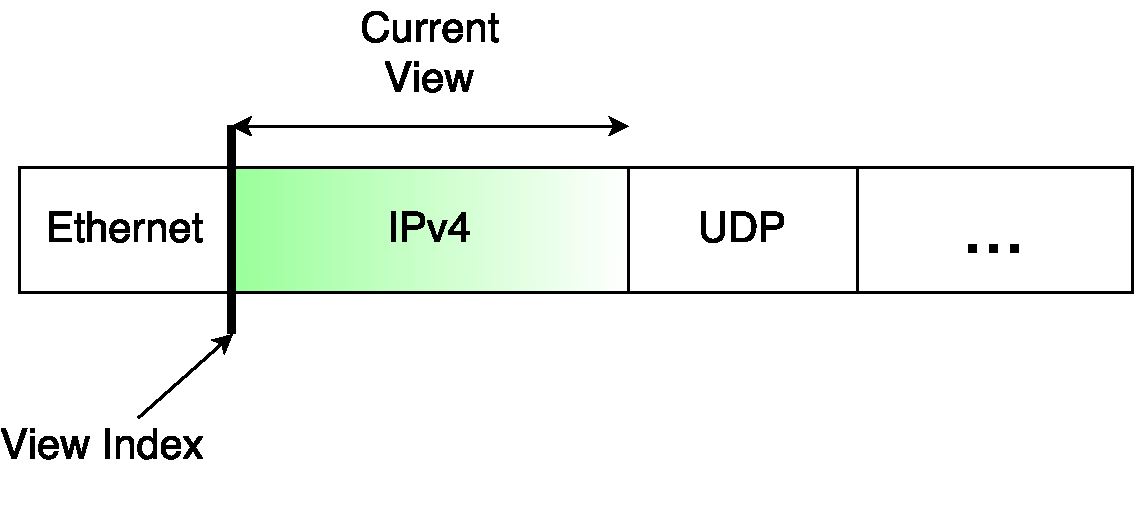
\includegraphics[width=.8\linewidth]{view3}
  \caption{When a decoder is finished working, it \textit{shifts} the view to
the next header. The shift moves the beginning of the view by the length of the
header -- 14 bytes.}
  \label{fg:view3}
\end{subfigure}%
\hfill
\begin{subfigure}[t]{.45\textwidth}
  \centering
  \includegraphics[width=.8\linewidth]{view4}
  \caption{The view shifts again by 20 bytes once the IPv4 decoder finishes.}
  \label{fg:view4}
\end{subfigure}
\caption{A demonstration of the decoding process in action.}
\label{fg:decoding}
\end{figure}

Each field in the header is discovered by information gathered by the layout
rule. The layout rule tells a decoder the location, or relative offset, of
each field from the beginning of the header (which is equivalent to the
beginning of the view). It also gives the length of each
field. From here, a decoder can go about discovering which bits form each
field as demonstrated in Figure \ref{fg:view2}.

When a decoder finishes, it \textit{shifts} the view, as seen in Figure
\ref{fg:view3}. The beginning of the view is moved by the length of header. The
view now starts one byte \textit{after} the previous header's final byte. All decoders are responsible for shifting the view in
preparation for the next decoder. Once the next decoder is reached, its view is
already on the header it decodes. When this next decoder finishes, it shifts the
view once again, as seen in Figure \ref{fg:view4}.

This process continues until the user decides that they are done decoding headers.

\subsection{Accessing Extracted Fields} \label{tut:decoder_access}

After extracting a field from a header it is likely that one wants the
\textit{value} of that extraction. To get the value of an extraction
the \textit{field access expression} (\ref{guide:field_access_expr}) is used. When
using the field names from an extract declaration in other operations, such as
the condition of an \texttt{if} statement, or an operand in addition, it is used to
mean the value of that field. That field name \textit{becomes} a field access
expression.

A typical operation on an ethernet header is determining which protocol
it encapsulates, i.e. the header which comes next. For that, the value of the \texttt{ethernet.type} field is required.
The following example demonstrates how to use the value of the \texttt{ethernet.type} extraction.

\begin{codepage}
\begin{lstlisting}
decoder start eth_d(ethernet)
{
  extract ethernet.dst;
  extract ethernet.src;
  // Use the type field to determine info on the next header.
  extract ethernet.type;
  // Using a field access expression with logical operator >=
  if (ethernet.type >= 0x600) {
    // Then type determines what header comes next.
  }
  else if (ethernet.type <= 0x05dc) {
    // Then type is the length of the entire packet.
  }
  // ...
}
\end{lstlisting}
\end{codepage}

The IEEE ethernet standard says that \texttt{ethernet.type} fields greater than or equal
to \texttt{0x600} indicate the next header's protocol \cite{eth_std}. Any \texttt{type}
fields less than \texttt{0x05dc} indicate the ethernet frame's length. Here, field access is used to compare \texttt{ethernet.type} to hexadecimal literals in an
\texttt{if-else} statement to determine the meaning of that field.

Field access values can also be used in arithmetic operations, comparison operations, bitwise operations, function calls,
and can be stored and assigned to variables. The following example presents
a trivial IPv4 decoder demonstrating some of these basic operations.

\begin{codepage}
\begin{lstlisting}
decoder ipv4_d(ipv4)
{
  // We actually need all fields to confirm the checksum later.
  extract ipv4.version_ihl; // Use this to get header length.
  extract ipv4.dscp_ecn;
  extract ipv4.len;
  extract ipv4.id;
  extract ipv4.fragment;
  extract ipv4.ttl;       // Use time-to-live to decrement
  extract ipv4.protocol;
  extract ipv4.checksum;
  extract ipv4.src;
  extract ipv4.dst;

  // Field values can be assigned to variables
  var pktlen : uint = ipv4.len;
  // Bitwise operations can be performed.
  var ihl : uint(8) = ipv4.version_ihl & 0x0f;
  // Shifts are valid as well.
  var version : uint(8) = ipv4.version_ihl >> 4;
  
  // More code to follow...
}
\end{lstlisting}
\end{codepage}

This example presents a solution for recovering non-byte aligned
fields. A bitwise-and (\ref{guide:bitwise_expr}) is used on \texttt{ipv4.version\_ihl}
with \texttt{0x0f} to recover the \texttt{ihl} field. The 
\texttt{ipv4.version\_ihl} is left-shift by 4 bits to get the \texttt{version} field.

Extractions can be passed to functions as well. A convenient use case is calculating the checksum for the IPv4 header. The following example extends the IPv4 decoder with a few more operations.

\begin{codepage}
\begin{lstlisting}
decoder ipv4_d(ipv4)
{
  // Code from before...
  
  // Calculate a checksum by calling a function.
  var checksum : uint(16) =
 	  ipv4_checksum(ipv4.version_ihl, ipv4.dscp_ecn, ipv4.len, 
                    ipv4.id, ipv4.fragment, ipv4.ttl, 
                    ipv4.protocol, ipv4.src, ipv4.dst);

  // Check the checksum against the header's checksum.
  if (checksum != ipv4.checksum)
	  drop;

  // Drop time-to-live expired packets.
  if (ipv4.ttl == 0)
    drop;

  set ipv4.ttl = ipv4.ttl - 1; // Decrement ttl.

  // The ttl has changed, so a new checksum must be calculated.
  set ipv4.checksum =
    ipv4_checksum(ipv4.version_ihl, ipv4.dscp_ecn, ipv4.len, 
                  ipv4.id, ipv4.fragment, ipv4.ttl, 
                  ipv4.protocol, ipv4.src, ipv4.dst);
}
\end{lstlisting}
\end{codepage}

Fields from the IPv4 header are passed to a function named \texttt{ipv4\_checksum} (whose definition is shown later in Section \ref{tut:learning_router}). The resulting checksum is compared against the current checksum using an \texttt{if} statement. If they do not compare equal, then the packet is dropped using the \texttt{drop} action.

Decrementing the time-to-live (\texttt{ipv4.ttl}) is another common operation. First the time-to-live is checked to see if it is \texttt{0}. If it is, then the packet's lifetime has expired and it will be dropped. If the packet is still valid, the field is decremented using simple subtraction and is set using the \texttt{set} action. More details on the \texttt{set} action can be found in Section \ref{tut:set_action}. Because a field has been changed in the IPv4 header, the checksum must be recalculated and set with the new checksum.

Field access expressions do have a number of limitations. The following example
demonstrates some of them.

\begin{codepage}
\begin{lstlisting}
decoder start eth_d(ethernet)
{
  // Error: Cannot use eth.type before its extracted.
  if (ethernet.type >= 0x600) { }

  extract eth.type;

  // Now that its been extracted ...
  // Error: Cannot assign to a field this way.
  ethernet.type = 0x800;
  // A set action must be used instead
  set ethernet.type = 0x800;
}

decoder ipv4_decode(ipv4)
{
  // Error: eth.type was not extracted by this decoder.
  if (ethernet.type == 0x800) { }
}
\end{lstlisting}
\end{codepage}

A field access expression can only be used \textit{after} an extract declaration
is made for that field. After all, it is impossible to recover the value of a
field which has not been extracted. By extensions, they cannot be used in
decoders which have not extracted that field. A decoder focuses on exactly one
header and has no knowledge of previous headers or extractions.

Field access expressions cannot be assigned to like a variable. To modify the
value of a field, a \texttt{set} action (\ref{guide:set_field}) must be used instead.

\subsection{Moving to Other Stages} \label{tut:decoder_next}

Once the user decides that they are finished extracting fields and performing operations on the current header, the user must decide where to send the packet next. One should recall from Chapter \ref{ch:pipeline_model} that decoding and
table matching stages can be chained together in a number of flexible ways.
A decoder can move a packet to another decoder, table, or it can forward/drop
the packet. It is up to the user to decide which is appropriate.

To move to another decoding stage, a \texttt{decode} action (\ref{guide:decode_action})
is used. The following example bridges the ethernet and IPv4 decoders
declared in earlier examples. The \texttt{match} statement is used to check if \texttt{ethernet.type} is equal to
\texttt{0x800}. If it is, then it confirms the next header is IPv4 and the \texttt{decode} action moves the packet to the IPv4 decoder.

\begin{codepage}
\begin{lstlisting}
decoder start eth_d(ethernet)
{
	extract ethernet.dst;
	extract ethernet.src;
	extract ethernet.type;
	if (ethernet.type >= 0x600)
	  	// The next header is IPv4 if the type field is 0x800.
	    match (ethernet.type) {
	      case 0x800: decode ipv4_d;
	    }
	// Do something else...
}

decoder ipv4_d(ipv4) { ... }
\end{lstlisting}
\end{codepage}

To transition to a table matching stage, a \texttt{goto} action (\ref{guide:goto}) (not
to be confused with a C-like \texttt{goto}) is used.

\begin{codepage}
\begin{lstlisting}
decoder ipv4_d(ipv4)
{
  extract ipv4.version_ihl;
  extract ipv4.protocol;
  extract ipv4.src;
  extract ipv4.dst;
  // Calculate internet header length (ihl).
  var ihl : uint(8) = (ipv4.version_ihl & 0x0f) * 4;
  // We apply the advance clause to shift our view by a given
  // number of bytes.
  goto t1 advance ihl;
}
\end{lstlisting}
\end{codepage}

In this example, the \texttt{goto} action sends the packet to a hypothetical table
named \texttt{t1}. Details about writing tables follows in Section \ref{tut:table}. The most important thing to notice from this example is the
\texttt{advance} clause.

Section \ref{tut:extract_how} explains that a decoder shifts the
\textit{view} of a packet before moving to the next stage. That shift is by the
length of the header. IPv4 headers are dynamic in length. Even though Steve does not
currently support extracting dynamic length fields, one must still account for
them. To correctly do this, the \texttt{advance} clause is applied to
explicitly shift the view by the given number of \textit{bytes}. The
\texttt{advance} clause may appear on both \texttt{goto} and \texttt{decode} actions.

The assumption is made that all headers are byte-aligned, therefore advancing by
a number of bytes (rather than bits) is appropriate. An
\texttt{advance} clause may only appear in a decoder, as decoders are the only
stage concerned with views.

A stage is \textit{complete} once it executes a \texttt{decode} or \texttt{goto} action, or
finishes executing without either action being executed. No actions written in a stage
\textit{after} a \texttt{decode} or \texttt{goto} action gets executed. These two actions are similar in
semantics to a return within a function. If no stage transition happens at all,
the packet exits the pipeline, as described in Section \ref{tut:pipeline_exit}.

\section{Tables} \label{tut:table}

The next stage is the table matching stage. 
Table stages classify packets into groups based on values found in a subset of that packet's extracted fields. In fact, it is a decision table, like those found in heuristics applications. This is done
through a mechanism known as a flow table defined by the OpenFlow standard
\cite{openflow_spec}.

\subsection{The Basic Table} \label{tut:basic_table}

Each flow table is comprised of three parts: 1) a name, 2) a \textit{key}, and
3) a set of \textit{flow entries}. Additionally, there may be three kinds of
flow tables: \textit{exact}, \textit{prefix}, and \textit{wildcard}. Steve
currently \textit{only} supports the exact flow table. Matching patterns are discussed later in this section.

The following example presents the basic form of a table named
\texttt{ethtype}. 

\begin{codepage}
\begin{lstlisting}
// The ethtype exact match table.
// This has a single key field: ethernet.type.
exact_table ethtype(ethernet.type)
{
	// Flow entries...
}
\end{lstlisting}
\end{codepage}

A table's \textit{key} is the set of fields, known as
\textit{key fields}, which that table looks at when classifying packets. They are the
equivalent of decision attributes. The \texttt{ethtype} table's key has a single
field -- \texttt{ethernet.type}.

Next, a set of \textit{flow entries} must be defined. Flow entries are like the
rules of a decision table. If a packet's fields match certain values, a
corresponding sequence of actions are performed.

To write a flow entry, a \textit{flow entry declaration}
(\ref{guide:tables}) is used. A flow entry declaration has two parts: 1) \textit{match
fields} and 2) an \textit{action sequence}. 

The following example presents two flow entries added to the \texttt{ethtype} table.

\begin{codepage}
\begin{lstlisting}
// The ethtype exact match table.
// This has a single key field: ethernet.type.
exact_table ethtype(ethernet.type)
{
	// This flow entry matches all packets whose
	// ethernet.type field equals 0x800.
	{ 0x800 } ->
	{
		// If it matches, send it to ipv4_d.
		decode ipv4_d;
	}
	// This is the miss case. It matches all packets
	// which do not match any other entry.
	miss ->
	{
		drop; // The drop action drops a packet.
	}
}
\end{lstlisting}
\end{codepage}

Match fields are values which
correspond to the table's key fields. When a packet is matched against a table,
the table compares the packet's fields with the match fields of each flow entry.
A packet \textit{matches} a flow entry, if each field (which is part of the
table's key) in the packet matches each corresponding match field in the flow entry. 

Match
fields appear as a comma-separated list of expressions in the brace-enclosed
block before the \texttt{->}. In the first flow entry, there is a single match field,
\texttt{0x800}, corresponding to the key field, \texttt{ethernet.type}.
All packets whose \texttt{ethernet.type} field is \texttt{0x800} will match
this flow entry. 

The second flow entry is a special entry known as the \textit{miss case}. The miss case uses the keyword \texttt{miss} rather than providing match fields. If no other flow entry in a table can match a packet, the miss case is used. A table may only have one flow entry. If one is not given, an implicit one exists which is the equivalent to the second flow entry in the example. That is, by default miss cases drop a packet.

There can be certain match patterns supported by a table: exact, prefix, and wildcard. Steve currently only handles the exact match pattern. The exact match pattern means the value of the field must be exactly equal to the value of the match field. A logical-xor of the two bit-patterns should produce a result equivalent to 0.

Following the \texttt{->} within the brace-enclosed block is
the action sequence. Actions change packets, action sets, and pipeline state.
Actions in this sequence are applied in
order if the packet matches the flow entry. The first flow entry has a single action, the \texttt{decode} action, which
will send the packet to the IPv4 decoder. The second flow entry also has a single action, the \texttt{drop} action, which drops a packet. Section \ref{tut:action}
describes many of these actions in greater detail.

In the earlier ethernet decoder example, a \texttt{match} statement was used to check that the \texttt{ethernet.type} field was equal to \texttt{0x800} before sending the packet to the IPv4 decoder. A table can be written to perform the same task. This is precisely what the \texttt{ethtype} table now does.

Now if the ethernet decoder from before is re-written, the same essential behavior is achieved.

\begin{codepage}
\begin{lstlisting}
decoder start eth_d(ethernet)
{
	extract ethernet.dst;
	extract ethernet.src;
	extract ethernet.type;
	goto ethtype;
}
\end{lstlisting}
\end{codepage}

Flow entries declared within a flow table, like in \texttt{ethtype}, are known
as \textit{initial flow entries}. They get installed before a Steve application
processes its first packet. Flow entries may also be added to a flow table after it has begun processing packets. An
example of adding flows can be found in Section \ref{tut:insert_flow_action}.

\subsection{A More Complex Table} \label{tut:complex_table}

The \texttt{ethtype} table from Section \ref{tut:basic_table} is only the most basic of flow tables. Flow tables can get
far more complicated.

Not all flow tables will match on a single field. In fact, most flow tables will
match on many fields. The following table declaration demonstrates this.

\begin{codepage}
\begin{lstlisting}
// The key fields are ipv4.fragment and ipv4.protocol.
exact_table ip_proto(ipv4.fragment, ipv4.protocol)
{
  // The fragment field of 0x0 indicated not fragmented packets.
  // The protocol field is 0x11 for UDP data.
  { 0x0, 0x06 } ->
  {
  	// Dispatch to the UDP Decoder.
  	decode udp_d;
  }
  // And so on...
}
\end{lstlisting}
\end{codepage}

This flow table tries to classify packets to determine which transport layer
protocol they use, and dispatches to the appropriate decoder.
Each flow entry restricts itself to only non-fragmented packets.

Flow entries may also have \textit{properties}. Properties are additionally
information stored alongside flow entries. Steve supports two properties:
timeout and egress.

If the timeout property is set, the flow entry will be ejected from its table
after a given number of seconds. This value may be between 1 and 65,535. The
egress property stores information about a port and becomes useful later on for learning
applications (see the learning switch example in Section
\ref{tut:learning_switch}).

The following example extends the previous \texttt{ip\_proto} table with a new flow entry using the timeout property.

\begin{codepage}
\begin{lstlisting}
exact_table ip_proto(ipv4.fragment, ipv4.protocol)
{
  // Previous flow entries...

  // The protocol field is 0x06 for TCP data.
  // A flow entry with a timeout is removed after X secs.
  [timeout = 1000]
  { 0x0, 0x06 } ->
  {
  	set ipv4.ttl = ipv4.ttl - 1; // Decrement time-to-live.
  	// Dispatch to the TCP Decoder.
  	decode tcp_d;
  }
  // And so on...
}
\end{lstlisting}
\end{codepage}

This flow entry sets the timeout property in the \textit{properties block}
preceding the usual flow entry declaration. The properties block is a
comma-separated list of properties.

The egress property is a little more tricky. It exists to support learning applications. An example of the egress property being used can be found in Section \ref{tut:output_action}.

Key fields are typically used to match specific values or sets of values. However, some flow tables may need fields extracted, yet not
necessarily care what the values of those fields are. For example, an IPv6 table
may want to decrement the hop-limit field which is roughly equivalent to time-to-live. This is a common operation, yet the table
does not care what the value of that field is (as long as it is greater than 0).
For these cases, there is the \texttt{requires} clause.

The \texttt{requires} clause gives a comma-separated sequence of fields which a table needs
extracted before being reached, but whose value is irrelevant. Each
\textit{required field} can be thought of as if it were a wildcard value (*).

The following example is a table which matches on one field and requires
\texttt{ipv6.next\_hop}.

\begin{codepage}
\begin{lstlisting}
// This table matches on the next header field by also
// requires that the hop limit have been extracted.
exact_table ipv6_proto(ipv6.next_header)
	requires (ipv6.hop_limit) // Requires clause.
{
  // 0x01 (ICMP) for the protocol field.
  { 0x01 } ->
  {
  	// Decrement the hop-limit.
  	set ipv6.hop_limit = ipv6.hop_limit - 1; 
  	// Dispatch to the ICMP Decoder.
  	decode icmp_d;
  }
  // And so on...
}
\end{lstlisting}
\end{codepage}



\subsection{The Reasoning Behind Flow Tables} \label{tut:why_tables}

\textit{What makes using a table different from decision structures like
if-else or match statements?} As anyone can tell, the \texttt{ethtype} table
presented in Section \ref{tut:basic_table} could have been written as a simple
match statement. What are the advantages?

\textit{Tables can match on one or more fields at once.} The more fields
required in the decision making process, the more complex using nested decision
structures gets. Tables can also match on a packet's ingress port
(\texttt{in\_port}) and physical ingress port (\texttt{in\_phys\_port}) fields
(described in Section \ref{tut:output_action}).

\textit{Tables can match on and use fields from different headers.} Unlike
decoders, tables have access to all extractions. The only limitation is that
field access only works on key fields or required fields. For example, the
following is a valid table.

\begin{lstlisting}
exact_table t1(in_port, in_phys_port, ethernet.dst, ipv4.dst)
{
	// ...
}
\end{lstlisting}

\textit{Flow entries can be added and removed from tables using the appropriate
actions.} This allows decision making on packets to change dynamically during
runtime. It is obviously impossible to add new branches to conditional
statements. The ability to add, or \textit{learn}, new entries allows us to
write applications which can evolve, such as learning switches and routers. An
example of adding flows can be found in Section \ref{tut:insert_flow_action}.

\textit{In some cases conditional statements are preferred over tables.} Table matching can be slow. If none of the advantages of using a table are needed, it is almost always more beneficial to use a conditional statement. Table matching is inherently slower than conditional branching and should actually be avoided when possible.

\section{Exiting the Pipeline} \label{tut:pipeline_exit}

Once a packet is finished going through decoders and flow tables, it must exit the pipeline.
A packet exits the pipeline when
a stage finishes executing, and does not send the packet to another stage. For
decoders, this means that its entire body has finished execution, but it has not
used a \texttt{decode} or \texttt{goto} action. In the following example, if
\texttt{ethernet.type} is not greater than or equal to \texttt{0x600}, pipeline
processing completes.

\begin{codepage}
\begin{lstlisting}
decoder start eth_d(ethernet)
{
	extract ethernet.type;
	if (ethernet.type >= 0x600) {
		// Do something...
	}
	// Do nothing. Packet exits pipeline.
}
\end{lstlisting}
\end{codepage}

If a \texttt{drop} action is applied like in the following example, pipeline processing
immediately stops and the packet is dropped.

\begin{codepage}
\begin{lstlisting}
decoder ipv4_d(ipv4)
{
  extract ipv4.ttl;

  // Drop packets whose time-to-live expired.
  if (ipv4.ttl == 0)
  	drop;
  // Nothing past here get's executed if ttl is 0...
}
\end{lstlisting}
\end{codepage}

For table stages, packets exit once a flow entry finishes executing its body and
does not apply a \texttt{goto} or \texttt{decode} action.

\begin{codepage}
\begin{lstlisting}
exact_table t1(eth.type) {
	{ 0x86dd } ->
	{
		// This will write the output action to the action set.
		write output flood;
		// Packet exits after the write action.
	}
}
\end{lstlisting}
\end{codepage}

Here, \texttt{t1}'s flow entry uses a \texttt{write} action (described in Section
\ref{tut:write_action}) to write an \texttt{output} action to the packet's action set.
Then, the packet exits the pipeline.

Once a packet completes pipeline processing, any actions written to its action
set get executed. A \textit{written} \texttt{output} action, when executed, modifies the
egress port field in the packet's context. This field ultimately decides where
the packet gets forwarded once its action set is done executing. If nothing is
written to this field, the packet is implicitly dropped.

\section{Ports} \label{tut:ports}

Steve supports limited access to ports.
There are two "kinds" of ports to consider when working with Steve: \textit{reserved ports} and
\textit{regular ports}.

\subsection {Reserved Ports} \label{tut:reserved_ports}

Reserved ports are ports which are always present on the system. Some ports may
be directly forwarded to using the \texttt{output} action. Other reserved ports are forwarded to implicitly by
other actions.

The following reserved ports may be forwarded to by the \texttt{output} action.

\begin{itemize}
\item \emph{All port}. Forwarding to the \textit{all} port will forward copies of the packet to
every port on the system.

\item \emph{Reflow port}. Forwarding to the \textit{reflow} port will send the packet back into
ingress processing. From there it will be processed again by the pipeline from
the beginning.

\item \emph{Flood port}. Forwarding to the \textit{flood} port sends copies of the packet to all
ports on the system \textit{except} the packet's ingress port.
\end{itemize}

Each of these reserved ports can be accessed using a reserved keyword. In the
following, the \texttt{output} action is used to send a packet to these three
ports.

\begin{codepage}
\begin{lstlisting}
all; // The all port
reflow; // The reflow port
flood; // The flood port

// Output action with these ports.
output all;
output reflow;
output flood;
\end{lstlisting}
\end{codepage}

The following reserved ports will be forwarded to by other actions.

\begin{itemize}
\item Packets are forwarded to the \textit{drop} port by the \texttt{drop} action.
Packets which are dropped get deleted.

\item Packets are forwarded to the \textit{controller} port when the \texttt{raise}
action is used. On the controller port sits a thread which will
execute event handlers (explained in Section \ref{tut:event}) on packet
contexts. Forwarding to the controller port is reserved only for exceptional
events.
\end{itemize}

\subsection{Regular Ports} \label{tut:regular_ports}

Regular ports are any ports on the system which are neither reserved nor are
guaranteed to be present. These ports can be split into \textit{physical} and
\textit{logical} ports. A physical port is a hardware interface on the system. A
logical port is a switch defined port which may map to multiple physical ports
and include additional abstractions.

Steve applications currently do not support a way of directly discovering all
these ports and their capabilities. Steve applications can indirectly "learn"
about these ports by observing the ingress ports of packets passing
through the pipeline.

There are two reserved keywords for getting the logical ingress port and physical ingress port of a packet.

\begin{codepage}
\begin{lstlisting}
in_port; // The logical ingress port.
in_phys_port; // The physical ingress port.

// Output action with these ports.
output in_port; // Send the packet back where it came from.
output in_phys_port;
\end{lstlisting}
\end{codepage}

\subsection{Port Variables} \label{tut:declared_ports}

Port variables can be used to \textit{remember} ports for later usage. They are
written using \textit{port declarations} (\ref{guide:port}).

\begin{codepage}
\begin{lstlisting}
Port p1; // Two port variables.
Port p2;
\end{lstlisting}
\end{codepage}

Other ports can be assigned to them. This does not copy the port. It just saves
a handle to that port inside the port variable. The following example demonstrates this.

\begin{codepage}
\begin{lstlisting}
p1 = in_port; // "Remember" a logical ingress port of a packet
p2 = in_phys_port; // and a physical ingress port.

output p1; // Forward to these ports.
output p2;
\end{lstlisting}
\end{codepage}

Here, the ingress ports of a packet are saved to port variables \texttt{p1} and \texttt{p2}. An \texttt{output} action may specify a port variable, in which case the packet is forwarded to the port whose handle is stored by the port variable.

\section{Actions} \label{tut:action}

Actions change packets, action sets, and pipeline state. Steve supports ten
actions with more anticipated in the future. Actions can be used in both
decoders and flows in Steve.

\subsection{Decode Action} \label{tut:decode_action}

The \texttt{decode} action is used to move a packet from the current stage to a
decoding stage. This action was present throughout a number of examples. As a
reminder, if the goal is to move to an IPv4 decoder named \texttt{ipv4\_d}, the
action would be written as:

\begin{lstlisting}
decode ipv4_d;
\end{lstlisting}

There is also an optional \texttt{advance} clause which is used if
the \textit{view} of the packet must be explicitly shifted by some special
number of bytes. For example, if the current decoder is for IPv4, and the next
decoder is named \texttt{udp\_d}, the action would be written as:

\begin{lstlisting}
decode udp_d advance (ipv4.version_ihl & 0x0f) * 4;
\end{lstlisting}

The \texttt{advance} clause may only be attached if the action is executed by a
decoder. Only decoders are responsible for view shifts.

\subsection{Goto Action} \label{tut:goto_action}

The \texttt{goto} action is used to move a packet from the current stage to a
table matching stage. If the goal is to move to a table named \texttt{t1}, the
action would be written as:

\begin{lstlisting}
goto t1;
\end{lstlisting}

Similar to the \texttt{decode} action, the \texttt{goto} action also supports an
optional advance clause. For example, if the current decoder is for IPv4, and
the table is named \texttt{t1}, the action would be written as:

\begin{lstlisting}
goto t1 advance (ipv4.version_ihl & 0x0f) * 4;
\end{lstlisting}

The \texttt{advance} clause may only be attached if the action is executed by a
decoder. Only decoders are responsible for view shifts.

\subsection{Output Action} \label{tut:output_action}

Output actions forward a \textit{copy} of the current packet to a port. As
mentioned earlier in Section \ref{tut:ports}, an \texttt{output} action may forward to a
number of ports named by keywords (\texttt{all}, \texttt{flood},
\texttt{reflow}, \texttt{in\_port}, \texttt{in\_phys\_port}), or may be
forwarded to a port saved by a port variable.

\begin{codepage}
\begin{lstlisting}
// Output to reserved ports.
output all; // The all port.
output reflow; // The reflow port.
output flood; // The flood port.

// Output to physical & logical ingress ports.
output in_port;
output in_phys_port;

// Output to port variables.
output p1; // Assuming there is is a port variable named 'p1'.
\end{lstlisting}
\end{codepage}

There are certain implications to the \texttt{output} action forwarding a copy of the packet. 
It means that multiple output actions can be written in
the same table or decoder. It also means that pipeline processing will continue
on the original packet.

The \textit{original} packet is forwarded once pipeline processing completes.
The destination port of the original packet is determined by a written \texttt{output}
action (described in Section \ref{tut:write_action}).

If a flow has its egress port property set, it is possible to output to that
port. In the following, a flow is inserted with its egress property set to the
current packet's ingress port. Within the flow body, the \texttt{output} action forwards
to the port saved by the egress port property.

\begin{codepage}
\begin{lstlisting}
// An inserted flow entry has its egress property set.
insert
[egress = in_port]
{ 0xffffffffffff } ->
{
	// We can output to egress.
	// This will forward all matching packets to the
	// current packet's ingress port.
	output egress;
}
into t1;
\end{lstlisting}
\end{codepage}

\subsection{Drop Action} \label{tut:drop_action}

A packet can be dropped by the Steve application using the \texttt{drop} action.
The \texttt{drop} action immediately ends the pipeline processing of a packet.

\begin{codepage}
\begin{lstlisting}
drop;
\end{lstlisting}
\end{codepage}

\subsection{Insert Flow Action} \label{tut:insert_flow_action}

Inserting flow entries into a table is a Steve action not explicitly supported
by the OpenFlow standard \cite{openflow_spec} though it is supported in
switches like OVS \cite{ovs_man_page} and is supported by POF \cite{pof, pof_fis, pof_impl}.

Flow entries can be inserted with constant key values and no properties. Here,
a flow entry is inserted into the table presented in Section
\ref{tut:complex_table}.

\begin{codepage}
\begin{lstlisting}
// Constant key values.
insert
{ 0x0, 0x89 } ->
{
  set ipv4.ttl = ipv4.ttl - 1;
  decode mpls_d;
}
into ip_proto;
\end{lstlisting}
\end{codepage}

They can also be inserted with field values of the current packet and with
optional properties.

\begin{codepage}
\begin{lstlisting}
// Dynamic key values
insert
[timeout = 1000, egress = in_port]
{ ipv4.fragment, ipv4.protocol } ->
{
  output egress;
}
into ip_proto;
\end{lstlisting}
\end{codepage}

In this case, the flow entry uses the \texttt{ipv4.fragment} and \texttt{ipv4.protocol}
fields of the current packet as values for the inserted flow entry's match fields.
It also sets the timeout to 1000 seconds and sets the \texttt{egress} property to the
current packet's \texttt{in\_port}, making the \texttt{output egress} action
valid.

If a new flow entry's match fields already exist in the table, the old flow
entry is replaced by the new flow entry. A miss case may be inserted into a
table as well.

\begin{codepage}
\begin{lstlisting}
insert
miss -> { output flood; }
into ip_proto;
\end{lstlisting}
\end{codepage}

\subsection{Remove Flow Action} \label{tut:remove_flow_action}

A flow entry can be removed from a table by providing match field values and the
name of the table to remove the flow entry from. This can be done with constant
values or dynamic field values of the current packet. If the flow entry with
those match field values does not exist, nothing is done.

\begin{codepage}
\begin{lstlisting}
// Removal with constant values.
remove { 0x0, 0x01 } from ip_proto;

// Or dynamic values.
remove {ipv4.fragment, ipv4.protocol} from ip_proto;
\end{lstlisting}
\end{codepage}

Miss cases can also be removed from tables. When a miss case is removed, it is
replaced by the default flow entry (which drops the packet).

\begin{codepage}
\begin{lstlisting}
// Removing a miss case.
remove miss from t1;
\end{lstlisting}
\end{codepage}

\subsection{Set Action} \label{tut:set_action}

A \texttt{set} action can be used to write to any extracted field within a
packet. For example, the time-to-live field from an IPv4 header may be set as
follows.

\begin{codepage}
\begin{lstlisting}
set ipv4.ttl = ipv4.ttl - 1;
\end{lstlisting}
\end{codepage}

The \texttt{set} action is only valid if the field access expression is valid in
that stage. For decoders, this means the field has to have been extracted first.
For tables, this means the field must be a key field or a required field. For
events, the field must be a required field.

\subsection{Write Action} \label{tut:write_action}

The context data structure described in Section \ref{context_desc} keeps an
\textit{action set}. Actions get written to the action set using the
\texttt{write} action. Written actions get executed once pipeline processing
completes and the packet enters egress processing (described in Section \ref{egress_desc}).

Only two actions may be written to a packet right now: \texttt{output} and \texttt{set}.

\begin{lstlisting}
// Writing a set action
write set ipv4.ttl = ipv4.ttl - 1;
// Writing an output action.
write output reflow;
\end{lstlisting}

The written \texttt{output} action has a slightly different semantic from the immediately
applied \texttt{output} action. When immediately applied, the \texttt{output} action forwards a
\textit{copy} of the packet. The written \texttt{output} action sets the egress port field
in the packet context when executed. This field ultimately decides where to forward the
\textit{original} packet.

\subsection{Clear Action} \label{tut:clear_action}

The \texttt{clear} action removes all actions from the context's action set.

\begin{lstlisting}
clear;
\end{lstlisting}

\subsection{Raise Action} \label{tut:raise_action}

A \texttt{raise} action is used to trigger an \textit{event}. Events are used to
handle exceptional situations described in Section \ref{tut:event}. Events
define \textit{event handlers} which operate on a packet context. A \texttt{raise} action
sends a copy of the packet context and the event handler to the controller port.
On the controller port sits a thread or program (implementation specific) which
executes these event handlers. A \texttt{raise} action is written as follows.

\begin{lstlisting}
// Assuming we have an event named "learn_event"
raise learn_event;
\end{lstlisting}

\section{Events} \label{tut:event}

An \textit{event stage} is a special processing stage outside the regular
run-to-completion pipeline. Event stages are used to deal with exceptional
situations. Event stages define \textit{event handlers} which are special
functions that operate on packet contexts. Event handlers do not execute and
block until completion. Blocking can severely bottleneck performance.

Specifically, inserting and removing flow entries are best executed inside
events. These operations are extremely expensive. They are atomic and require
locking tables in multi-threaded architectures.

An event is \textit{raised} using the \texttt{raise} action explained in Section
\ref{tut:raise_action}. When an event is raised, the packet context and event
handler are forwarded to the reserved controller port. On the controller port
awaits a thread or program which will execute these event handlers as they are
received.

To write an event handler, an \textit{event declaration}
(\ref{guide:event}) is used. Event declarations have a \texttt{requires} clause, just
like tables. An event may only be raised if all fields listed in its
\texttt{requires} clause have been extracted.

The following example presents a simple, nonsense event declaration. Here,
the event requires the \texttt{ethernet.src} and \texttt{ethernet.type} fields
be extracted. Inside the event, any statements (such as if, match,
assignment, variable declarations, etc.) and any actions described in Section
\ref{tut:action}.

\begin{codepage}
\begin{lstlisting}
// A dummy event.
event e1
	requires(ethernet.src, ethernet.type)
{
	if (ethernet.type == 0x800) {
		// Do something...
	}
	else if (ethernet.src > 0x00_12_34_56_78_9a) { }
	var x : uint(48) = 0;
	set ethernet.src = x;
	output reflow;
	// Perform some other actions...
}
\end{lstlisting}
\end{codepage}

An important thing to know is that a \textit{copy} of the context is operated on
by an event handler. Any changes made in the event handler does not modify the
original packet or its context. An event handler may be executed immediately
after a \texttt{raise} action is used, or it may be executed asynchronously. The decision
is Flowpath runtime (\ref{ch:flowpath}) implementation specific and the user should not
rely on one or the other being the case.

It is important to note that this feature is actually completely contrary to OpenFlow semantics
\cite{openflow_spec}. Typically, a completely independent program called a \textit{controller} defines event
handlers. That program, which resides on the control plane, waits on the controller port for packets to process.
Steve allows those event handlers to be defined and executed on the data plane instead.

The advantage here is that Steve events are written as part of the Steve
application and are thus subject to the same semantic, logical, and safety
guarantees applied to other pipeline stages. Additionally, it strips the latency associated with communicating through an external controller to get certain operations done.

\section{Examples} \label{tut:examples}

This section provides three basic network applications: a MAC learning switch, an IPv4 learning switch, a stateless TCP/UDP firewall, and a
wire using language features taught during this tutorial.

\subsection{The MAC Learning Switch} \label{tut:learning_switch}

The MAC (ethernet) learning switch forwards packets based on their MAC addresses. Learning switches exploit the likelihood that a
path towards a device with that source MAC address exists through
the port the packet entered on. The learning switch keeps track of this information by maintaining a lookup table. This lookup table maps a MAC address to a port which likely connects to the respective device. 

Over time, the switch learns these MAC addresses by observing source MAC addresses and ingress ports of packets. The switch forwards packets by
looking at the destination address and checking if it has learned that MAC
address yet. If it has not learned the address, it floods the packet. This prevents the need to constantly flood packets on all ports.

The first step in writing any Steve application is defining the layouts. A
learning switch only concerns itself with the ethernet header.

\begin{codepage}
\begin{lstlisting}
// This layout describes the ethernet header.
layout ethernet
{
	dst  : uint(48); // This is 48 bits long.
	src  : uint(48); // This is 48 bits long.
	type : uint(16); // This is 16 bits long.
}
\end{lstlisting}
\end{codepage}

The next step is the ethernet decoder. Since this application is only concerned with the
ethernet header, there is no reason to extract
\texttt{ethernet.type}.

\begin{codepage}
\begin{lstlisting}
decoder start eth_d(ethernet)
{
	// Extract the src and dst MAC addresses; type isn't needed.
	extract ethernet.dst;
	extract ethernet.src;
	goto learn; // We proceed to the first table stage.
}
\end{lstlisting}
\end{codepage}

From here, the application will need two tables: a learning table and a forwarding table.
Using two tables will be typical of almost all learning applications. Both
tables will start out with nothing but a miss case. After all, before an
application runs, it has not learned anything yet. The first few packets will
certainly match against these miss cases.

The learning table is responsible for observing and learning MAC addresses, therefore it will match on \texttt{ethernet.src}. This table will raise an event which will
cause new flow entries to be inserted into both tables.  A flow entry will be installed into this
table to prevent the same \texttt{ethernet.src} from being learned multiple
times.

\begin{codepage}
\begin{lstlisting}
// This packet will cause new addresses to be learned.
exact_table learn(ethernet.src)
{
  miss ->
  {
  	// We raise an event to learn the appropriate flow entries.
  	raise learn_mac;
    goto forward; // Then send to the forwarding table.
  }
}
\end{lstlisting}
\end{codepage}

To insert the necessary flow entries, the \texttt{learn} table raises an event
called \texttt{learn\_mac}. The contents of this event will be presented a little later in this section.
After this event is raised, the learning table sends the packet to the
forwarding table.

\begin{codepage}
\begin{lstlisting}
// This table ultimately decides which packet to forward on.
exact_table forward(ethernet.dst)
{
  // Flood any packet which hasn't been learned yet.
  miss -> { output flood; }
}
\end{lstlisting}
\end{codepage}

The forwarding table contains flow entries which map MAC addresses to ports. It will lookup destination MAC addresses and ultimately forward the packet. The forwarding table thus
matches on \texttt{ethernet.dst}. If the table has yet to learn the MAC address, it floods the packet to all ports.


The \texttt{learn\_mac} event is where the actual
learning happens, and is thus the most important snippet of code in this
application. The one extraction this event will need is \texttt{ethernet.src}.
This is the MAC address the tables will be learning.

\begin{codepage}
\begin{lstlisting}
// This event will do the "learning" through flow inserts.
event learn_mac
	requires(ethernet.src) // It requires the src MAC
{
	// First we insert the src of the packet
	// into the learn table so we don't keep
	// trying to learn something we already have.
	insert
	[timeout = 60]
	{ ethernet.src } -> { goto forward; }
	into learn;

	// Next we insert the src of the current packet
	// into the forward table.
	//
	// The forward table matches on the dst field of a packet.
	// What we are doing is saying any packet whose dst is equal
	// to this packet's src is forwarded to this packet's
	// ingress port.
	insert
	[timeout = 60, egress = in_port]
	{ ethernet.src } ->
	{
		// We set the egress property to the current
		// packet's in_port. Future packets will be forwarded to
		// the current packet's ingress port.
		output egress;
	}
	into forward;
}
\end{lstlisting}
\end{codepage}



This event will insert two flow entries. The first flow entry is inserted into
the learning table. This entry prevents the same MAC address from raising the
\texttt{learn\_mac} event more than once. Instead, the new flow entry sends the
packet directly to the forwarding table.

The second inserted flow entry is where the application actually learns the new MAC
address. It is here where the application establishes a set of MAC address to port mappings.

One must first note that \texttt{forward} matches on \texttt{ethernet.dst}. Here, the application inserts a
flow entry with the \textit{current} packet's \texttt{ethernet.src} value into
\texttt{forward}. This means that all \textit{future} packets whose
\texttt{ethernet.dst} equals the \textit{current} packet's \texttt{ethernet.src}
will match this inserted flow entry. The egress property is set equal to the
\textit{current} packet's ingress port. The flow entry's body subsequently uses
\texttt{output egress} to output matched packets to the current packet's ingress port. Once this is done, the MAC address to port mapping is complete.

To summarize, the second flow entry ensures that all future packets whose
\texttt{ethernet.dst} field match the current packet's \texttt{ethernet.src}
field will be forwarded to the current packet's ingress port.

\subsection{The IPv4 Learning Switch} \label{tut:learning_router}

The IPv4 learning switch is not too different from the MAC learning switch. Instead of
learning and forwarding from MAC addresses, this application will use IPv4
addresses.

To start, the layouts must be defined. The ethernet layout
from the learning switch in Section \ref{tut:learning_switch} can be reused. 
In addition, the IPv4 layout is also needed.

\begin{codepage}
\begin{lstlisting}
// The layout needed to decode ipv4 headers.
layout ipv4
{
  version_ihl : uint(8);
  dscp_ecn    : uint(8);
  len         : uint(16);
  id          : uint(16);
  fragment    : uint(16);
  ttl         : uint(8);
  protocol    : uint(8);
  checksum    : uint(16);
  src         : uint(32);
  dst         : uint(32);
}
\end{lstlisting}
\end{codepage}

An ethernet decoder is needed again, however, this time the MAC
addresses are not needed. Instead, the \texttt{ethernet.type} field is needed to confirm
this is an IPv4 packet. If it is, the packet is sent to the IPv4 decoder.

\begin{codepage}
\begin{lstlisting}
decoder start eth_d(ethernet)
{
	extract ethernet.type;
	if (ethernet.type >= 0x600)
	  	// The next header is IPv4 if the type field is 0x800.
	    match (ethernet.type) {
	      case 0x800: decode ipv4_d;
	    }
	// If its not IPv4, processing ends and the packet is
	// implicitly dropped.
}
\end{lstlisting}
\end{codepage}

The IPv4 decoder will need to extract all of its fields to calculate a checksum. It will need \texttt{ipv4.src} and \texttt{ipv4.dst} in
order to learn them. It will need \texttt{ipv4.version\_ihl} to
correctly advance past the IPv4 header and \texttt{ipv4.ttl} to decrement.

\begin{codepage}
\begin{lstlisting}
decoder ipv4_d(ipv4)
{
  // Need all fields to confirm the checksum.
  extract ipv4.version_ihl; // Use this to get header length.
  extract ipv4.dscp_ecn;
  extract ipv4.len;
  extract ipv4.id;
  extract ipv4.fragment;
  extract ipv4.ttl;       // Use time-to-live to decrement
  extract ipv4.protocol;
  extract ipv4.checksum;
  extract ipv4.src;
  extract ipv4.dst;

  // Calculate a checksum.
  var checksum : uint(16) =
     ipv4_checksum(ipv4.version_ihl, ipv4.dscp_ecn, ipv4.len, 
                   ipv4.id, ipv4.fragment, ipv4.ttl, 
                   ipv4.protocol, ipv4.src, ipv4.dst);

  // Check the checksum against the header's checksum.
  if (checksum != ipv4.checksum)
    drop;

  // Drop time-to-live expired packets.
  if (ipv4.ttl == 0)
    drop;

  set ipv4.ttl = ipv4.ttl - 1; // Decrement ttl.

  // The decoder changed the ttl. It must set a new checksum.
  set ipv4.checksum =
    ipv4_checksum(ipv4.version_ihl, ipv4.dscp_ecn, ipv4.len, 
                  ipv4.id, ipv4.fragment, ipv4.ttl, 
                  ipv4.protocol, ipv4.src, ipv4.dst);

  // Proceed to the learn table after advancing by ihl
  goto learn advance (ipv4.version_ihl & 0x0f) * 4;
}
\end{lstlisting}
\end{codepage}

Here, the decoder will drop all packets with bad checksums or whose time-to-live has expired. It will decrement \texttt{ipv4.ttl} and compute a new checksum before sending the packet to table matching. The function used to calculate the checksums is as follows.

\begin{codepage}
\begin{lstlisting}
def ipv4_checksum(vihl:uint(8), dscp_ecn: uint(8), 
  len : uint(16), id : uint(16), frag : uint(16), 
  ttl : uint(8), proto : uint(8), src : uint(32), 
  dst : uint(32)) -> uint(16)
{
  // Merge fields into 16-bit values.
  var merge1 : uint(16) = vihl << 8;
  merge1 = merge1 | dscp_ecn;

  var merge2 : uint(16) = ttl << 8;
  merge2 = merge2 | proto;

  // Split fields int 16-bit values.
  // The upper 16 bits.
  var split_src1 : uint(16) = src >> 16; 
  // The lower 16 bits.
  var split_src2 : uint(16) = src & 0x0000_ffff;

  // The upper 16 bits.
  var split_dst1 : uint(16) = dst >> 16;
  // The lower 16 bits.
  var split_dst2 : uint(16) = dst & 0x0000_ffff;

  // Calculate the checksum.
  // Store the accumulated sum of each field.
  var acc : uint(32) = 0;
  acc = acc + merge1 + len + id + frag + merge2 +
        split_src1 + split_src2 + split_dst1 + split_dst2;

  // Perform the 1's complement sum wraparound.
  var acc1 : uint(16) = acc >> 16; // The upper 16 bits.
  var acc2 : uint(16) = acc & 0x0000_ffff; // Lower 16 bits.
  acc2 = acc1 + acc2; // End around carry.
  acc2 = acc2 ^ 0xffff_ffff; // Get the 1's compliment.
  return acc2;
}
\end{lstlisting}
\end{codepage}


Two tables are needed just like in the learning switch example. These tables 
are for learning and routing. They will start with only miss cases. 

Here, the \texttt{learn} table matches on \texttt{ipv4.src}. It will raise the event which
causes the IPv4 address to be learned. It will also prevent the same IPv4 address
from being learned multiple times.

\begin{codepage}
\begin{lstlisting}
// The learn table will cause addresses to be learned.
exact_table learn(ipv4.src)
{
	miss ->
	{
		// It raises the event which will insert new flow entries.
		raise learn_ip;
		goto routing;
	}
}
\end{lstlisting}
\end{codepage}

The routing table matches on \texttt{ipv4.dst}. This table will establish IPv4
address to port mappings. It will forward all packets whose destination IPv4
address it has learned. Any IPv4 addresses not yet learned are flooded by
default.

\begin{codepage}
\begin{lstlisting}
// This ultimately decides where to forward packets based on
// their destination IP.
exact_table routing(ipv4.dst)
{
	miss ->
	{
		output flood; // Flood on all unlearned addresses.
	}
}
\end{lstlisting}
\end{codepage}

Lastly, the \texttt{learn\_ip} event must be defined. It is
largely the same as the \texttt{learn\_mac} event from the learning switch.

\begin{codepage}
\begin{lstlisting}
// This event handles the actual "learning."
event learn_ip
	requires(ipv4.src) // It will learn src IP addresses.
{
	// This first entry prevents the same address from causing
	// this event twice. It sends the packet straight to routing.
	insert
	[timeout = 30]
	{ ipv4.src } -> { goto routing; }
	into learn;

	// This establishes the IP address to port mapping.
	// Any packet whose dst address matches the current packet's
	// src address will be forwarded to the current packet's
	// ingress port.
	insert
	[timeout = 30, egress = in_port]
	{ ipv4.src } ->
	{
		output egress;
	}
	into routing;
}
\end{lstlisting}
\end{codepage}

The first inserted flow entry prevents the same IPv4 address from being learned
more than once. The second insert flow entry inserts the routing rule into the
routing table. Any packet whose \texttt{ipv4.dst} is equal to the current
packet's \texttt{ipv4.src} will be forwarded to the current packet's ingress
port.

\subsection{A Stateless Firewall Extension} \label{tut:firewall}

Routers will often have stateless firewalls or packet filters installed. 
Stateless firewalls maintain a set of rules. These rules only allow packets 
through if their destination matches certain port numbers. A possible use 
case is a firewall set up before a web server. This firewall will block all 
non-HTTP/HTTPS requests.

It is possible to define this kind of transport layer firewall in Steve. This firewall will be an extension to the IPv4 switch from Section \ref{tut:learning_router}.

The \texttt{ethernet} and \texttt{ipv4} layouts from the Ipv4 switch will remain the same. In addition to these, two transport layer layouts must also be defined: the UDP and the TCP layouts.

The UDP header \cite{udp_std} contains four fields: source port, destination port, header length, and checksum. The UDP layout is defined as follows.

\begin{codepage}
\begin{lstlisting}
layout udp
{
  src      : uint(16);
  dst      : uint(16);
  len      : uint(16);
  checksum : uint(16);
}
\end{lstlisting}
\end{codepage}

The TCP header \cite{tcp_std} contains eight fields: source port, destination port, a sequence number, an acknowledgment number, control information (combining data offset and TCP flags), a window size, a checksum, and an urgent pointer. The dynamic length options field is excluded. The TCP layout is defined as follows.

\begin{codepage}
\begin{lstlisting}
layout tcp
{
  src : uint(16);
  dst : uint(16);
  ack : uint(32);
  seq : uint(32);
  // control: TCP len: 0-3, Reserved: 4-9, Flags: 10-15
  control : uint(16); 
  window : uint(16);
  checksum : uint(16);
  urgent_ptr : uint(16);
  // Ignore options.
}
\end{lstlisting}
\end{codepage}

The final line of the IPv4 decoder, \texttt{ipv4\_d}, from Section \ref{tut:learning_router} will be replaced so that the packet is now sent to a TCP or UDP decoder rather than to the learning table.

\begin{codepage}
\begin{lstlisting}
decoder ipv4_d(ipv4)
{
  // ipv4 decoder code from before...
  
  // Changing the final line to dispatch to new decoders.
  var hdr_len : uint(8) =  (ipv4.version_ihl & 0x0f) * 4;
  match (ipv4.protocol) {
    case 0x06: decode tcp_d advance hdr_len;
    case 0x11: decode udp_d advance hdr_len;
  }
}
\end{lstlisting}
\end{codepage} 


A \texttt{match} statement is used on the \texttt{ipv4.protocol} field. If it is equal to \texttt{0x06}, then the next header is TCP. If it is \texttt{0x11}, then the next header is UDP. A flow table may have also been used to make this decision, however, here it is not strictly necessary.

The TCP and UDP decoders are trivial. All this firewall is concerned with is their destination port. This firewall will ignore performing checksum validation for the sake of simplicity. 

\begin{codepage}
\begin{lstlisting}
decoder udp_d(udp)
{
  extract udp.dst;
  goto udp_filter advance;
}

decoder tcp_d(tcp)
{
  extract tcp.dst;
  goto tcp_filter;
}
\end{lstlisting}
\end{codepage}

Once the destination port is extracted, each decoder will send the packet to 
a filtering table. Here, the \texttt{advance} clause is not attached to the 
\texttt{goto tcp\_filter} action. Normally, it would be, however, if one does 
not expect another decoder later on, it is acceptable to leave it off.

\begin{codepage}
\begin{lstlisting}
// Only learn/route if the port# is 80 or 443
exact_table udp_filter(udp.dst)
{
  { 80 } -> { goto learn; }
  { 443 } -> { goto learn; }
}

exact_table tcp_filter(tcp.dst)
{
  { 80 } -> { goto learn; }
  { 443 } -> { goto learn; }
}
\end{lstlisting}
\end{codepage}

Each filtering table will only allow packets whose destination ports are \texttt{80} (HTTP) and \texttt{443} (HTTPS) to be forwarded. All others are dropped. Additional flow entries may be added depending on the purpose of the firewall. It is best practice to defined the minimum \textit{allowed} ports rather than those ports that need blocked. From here, the firewall will send to the learning and routing tables defined earlier in Section \ref{tut:learning_router}.

\subsection{The Wire} \label{tut:wire}

A full-duplex wire is a network application which has two ports. It receives from one port
and outputs out of the other port. The only caveat is that the application is
not aware of the ports comprising the wire at first. It must learn that those
ports exist.

This example demonstrates a number of more unintuitive features related to
ports. First, two uninitialized port variables named \texttt{p1} and
\texttt{p2} are declared. Uninitialized port variables always compare equal to 0.

\begin{codepage}
\begin{lstlisting}
// Our uninitialized port variables.
// These will compare equal to 0 at first
Port p1; .
Port p2;
\end{lstlisting}
\end{codepage}

The ethernet layout from prior examples can be used to write a starting decoder. The
special thing about this decoder is that it does not care about any of the fields.
It only needs the ingress port.

\begin{codepage}
\begin{lstlisting}
decoder start eth_d(ethernet)
{
	// We use the port variables, p1 and p2, to "remember" ports.

	// Whenever a packet is handled, check if p1 and p2 are set.
	// If neither are, set p1 equal to the ingress port.
	if (p1 == 0 && p2 == 0)
		p1 = in_port;
	// If p1 is set, and p2 isn't, set p2 to the ingress port.
	else if (p1 != 0 && p2 == 0)
		p2 = in_port;

	// Now we decide which packet to forward to.
	// If the ingress port is p1, and p2 is set, forward to p2.
	if (in_port == p1 && p2 != 0)
		output p2;
	// If the ingress port is p2, and p1 is set, forward to p1.
	if (in_port == p2 && p1 != 0)
		output p1;

	// If both are not set yet, do nothing and implicitly drop.
}
\end{lstlisting}
\end{codepage}

Here, the two port variables are used to remember what ports exist. The decoder
looks at the ingress port and saves it into one of the two variables. Once two
ports are "remembered," forwarding decisions can be made. If a packet comes from
\texttt{p1}, then it is forwarded through the only other port, \texttt{p2}, and
vice-versa. Before both ports are saved, since no other actions are applied, the
packet finishes pipeline processing and gets dropped.

For a full-duplex wire, it is always advised that one testing packet is sent to both interfaces before any packets are handled, to ensure the application is immediately aware of both ports.
